\notechapter{N-20260417}{Green Formula, Conservative Fields, and the Planar Stokes Principle}


\section{Green's theorem}

For a positively oriented simple closed curve $C=\partial D$ and sufficiently smooth $P,Q$,
\[
  \oint_C P\,dx+Q\,dy
  =\iint_D \left(\frac{\partial Q}{\partial x}-\frac{\partial P}{\partial y}\right)\,dA.
\]
The left side is circulation along the boundary; the right side is accumulated local rotation over the region.

\begin{figure}[H]
\centering
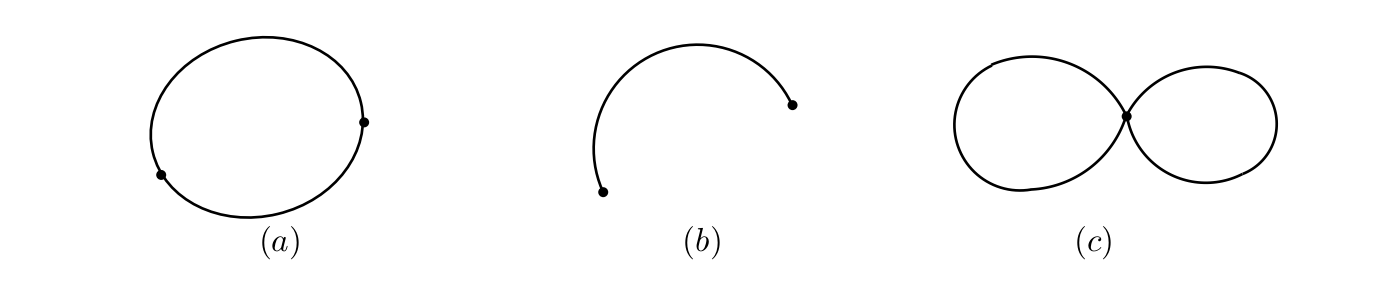
\includegraphics[width=0.82\textwidth,height=0.74\textheight,keepaspectratio]{figures/notes-md/N-20260417/N-20260417-fig-01-green-simple-closed-curves.png}
\caption{Simple closed curves and non-simple closed curves in the statement of Green's theorem.}
\end{figure}


\section{Path independence}

A vector field $F=(P,Q)$ is conservative if there exists $\phi$ such that
\[
  \nabla \phi=F.
\]
Then
\[
  \int_C P\,dx+Q\,dy=\phi(B)-\phi(A)
\]
for any path from $A$ to $B$.  On a simply connected region, $P_y=Q_x$ is the usual test for conservativity.

\begin{figure}[H]
\centering
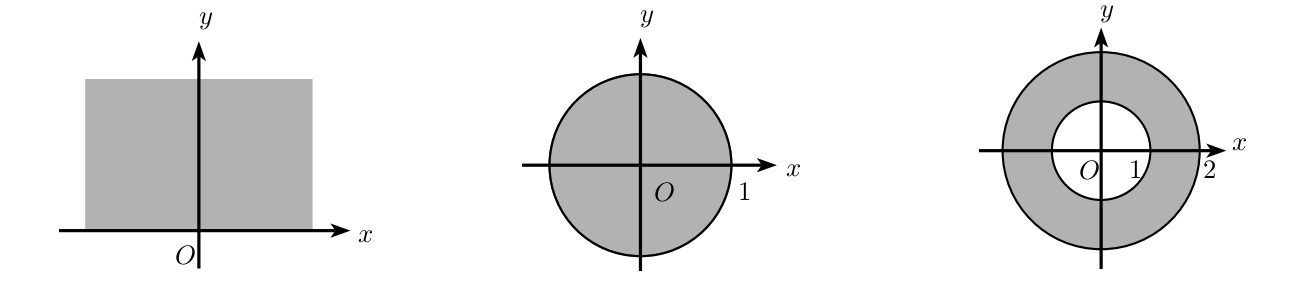
\includegraphics[width=0.82\textwidth,height=0.74\textheight,keepaspectratio]{figures/notes-md/N-20260417/N-20260417-fig-02-green-simply-connected-regions.png}
\caption{Simply connected and multiply connected plane regions.  The distinction matters for path independence and conservative fields.}
\end{figure}




\section{Expanded synthesis and advanced context}

Green's theorem is Stokes' theorem in the plane.  It says that the integral of a differential form over a boundary equals the integral of its derivative over the region.  This is the conceptual bridge to surface flux, Gauss' theorem, and the general Stokes theorem.



\paragraph{Expanded synthesis.}
For this chapter, the elementary material should be read as a study of what remains invariant when coordinates change. The earlier sections (`Green's theorem`, `Path independence`, `Higher viewpoint`, `Expanded Green-theorem proof idea`) compute with arrays, bases, pivots, determinants, or eigenvectors; the deeper object is a linear map together with the spaces it acts on. A matrix is a representation of that map after bases have been chosen. This is why formulas such as
\[
  A' = P^{-1}AP,\qquad \widetilde A = T^{-1}AS
\]
are not cosmetic: they distinguish an intrinsic morphism from a coordinate description.

The structural hierarchy is as follows. Kernels record what a map forgets, images record what it reaches, cokernels record obstructions to solvability, and quotients record information after an equivalence has been imposed. Determinants act on the top exterior power and therefore measure oriented volume; traces are invariant under cyclic rearrangement and become characters in representation theory; adjoints depend on an inner product and lead to self-adjoint spectral theory.

A useful way to return to the computations is to ask, for every formula, which invariant it is measuring. Row reduction measures rank and kernel; diagonalization measures decomposition into invariant subspaces; Gram--Schmidt measures orthogonal projection; positive definiteness measures ellipsoid geometry; tensor notation measures how components transform. The elementary methods are therefore the finite-dimensional laboratory in which duality, quotienting, functoriality, and spectral decomposition can be seen clearly.


\section{Expanded Green-theorem proof idea}

For a rectangle, Green's theorem can be checked by the fundamental theorem of calculus.  The $Q\,dy$ part accumulates horizontal changes in $Q$, and the $P\,dx$ part accumulates vertical changes in $P$ with the opposite sign.

Summing small rectangles makes interior boundary contributions cancel, leaving only the outer boundary.

This cancellation is the core of all Stokes-type theorems.  Local boundary pieces cancel in pairs; only the global boundary remains.

\begin{figure}[H]
\centering
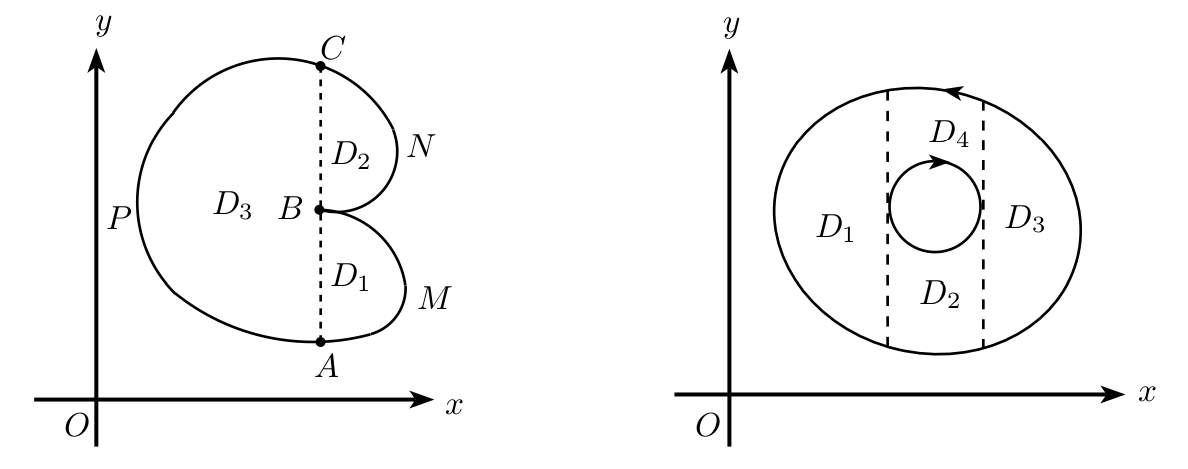
\includegraphics[width=0.82\textwidth,height=0.74\textheight,keepaspectratio]{figures/notes-md/N-20260417/N-20260417-fig-04-green-subdivision-boundary-cancellation.png}
\caption{Subdivision by auxiliary arcs: internal boundary contributions cancel, leaving only the outer boundary.}
\end{figure}


\section{Conservative fields and topology}

The condition $P_y=Q_x$ says that local curl is zero.  On a simply connected region, this implies the field is conservative.  On a region with a hole, it may fail.  The standard example is
\[
  F(x,y)=\left(-\frac{y}{x^2+y^2},\frac{x}{x^2+y^2}\right)
\]
on $\mathbb R^2\setminus\{0\}$.  Its curl is zero away from the origin, but circulation around the unit circle is $2\pi$.

\section{Elementary-to-advanced bridge: closed forms and exact forms}

For a plane vector field $F=(P,Q)$, the form
\[
  \omega=P\,dx+Q\,dy
\]
is closed when
\[
  d\omega=(Q_x-P_y)\,dx\wedge dy=0.
\]
It is exact when $\omega=df$ for some potential $f$.

Exact implies closed because $d^2=0$.  The converse depends on topology.  On simply connected domains in the plane, closed one-forms are exact.  On a punctured plane, this can fail.

\section{Elementary-to-advanced bridge: de Rham cohomology}

The first de Rham cohomology group is
\[
  H^1_{dR}(M)=\frac{\ker(d:\Omega^1(M)\to\Omega^2(M))}{\operatorname{im}(d:\Omega^0(M)\to\Omega^1(M))}.
\]
It measures closed one-forms modulo exact ones.  If $H^1_{dR}(M)=0$, every closed one-form is exact.

The standard form on the punctured plane,
\[
  \omega=\frac{-y\,dx+x\,dy}{x^2+y^2},
\]
is closed but not exact, because
\[
  \int_{S^1}\omega=2\pi.
\]
This integral detects the hole at the origin.

\section{Elementary-to-advanced bridge: Green's theorem as Stokes theorem}

Green's theorem says
\[
  \oint_{\partial D}P\,dx+Q\,dy
  =\iint_D (Q_x-P_y)\,dx\,dy.
\]
In differential-form notation, this is
\[
  \int_{\partial D}\omega=\int_D d\omega.
\]
This is exactly Stokes' theorem in dimension two.

The original path-independence tests therefore belong to a broad principle: boundary integrals measure the integral of a derivative over the interior.

\section{Elementary-to-advanced bridge: harmonic forms}

On a compact Riemannian manifold, each de Rham cohomology class has a unique harmonic representative.  A harmonic form satisfies
\[
  \Delta \omega=0,
\]
where $\Delta$ is the Hodge Laplacian.  This is Hodge theory.

For elementary vector calculus, the hint is this: fields can be decomposed into gradient-like, curl-like, and harmonic parts.  The harmonic part records topology.  This is the high-level continuation of conservative-field tests.

% Second-pass deepening for waves 2-4: wave 4 part 3
\section{Second-pass deepening: circulation as obstruction to a potential}

A field can have zero curl locally but still fail to have a global potential.  The punctured-plane form
\[
  \omega=\frac{-y\,dx+x\,dy}{x^2+y^2}
\]
is the standard example.  It is locally $d\theta$, but $\theta$ cannot be chosen as a single-valued global function on the punctured plane.

The integral
\[
  \int_{S^1}\omega=2\pi
\]
measures winding around the missing point.  Thus a line integral can detect topology.  This is the serious meaning behind the elementary warning that $P_y=Q_x$ is not enough on a domain with holes.

\section{Second-pass deepening: Green's theorem as cancellation of internal boundaries}

One way to understand Green's theorem is to subdivide a region into many small rectangles.  The boundary integrals over internal edges cancel because each internal edge is traversed twice in opposite directions.  Only the outer boundary remains.  This cancellation principle survives in chain complexes, singular homology, and general Stokes theorem.

The elementary proof by rectangles therefore already contains the algebraic identity
\[
  \partial^2=0,
\]
namely: the boundary of a boundary cancels.
